\documentclass{beamer}
\usepackage[ngerman]{babel}
\usepackage[utf8]{inputenc}
\usepackage{setspace} 
\usepackage{amsmath}
\usepackage{amsthm}
\usepackage{pgfplots}
\usepackage{siunitx}
\usepackage{eurosym}
\sisetup{locale = DE}
\sisetup{per-mode=fraction}
% Lade Beamer Stile
\usepackage{beamerthemesplit}
\usetheme{Rochester}
\usecolortheme{crane}
\setbeamercolor{bgcolor}{fg=black,bg=green!15!white}
\title{Beispielaufgabe Wasserkocher}
\subtitle{Forschungsfrage}
\author{Heiko Schröter}
\date{\today}

\setbeamertemplate{enumerate item}{\alph{enumi})}
\newtheorem{satz}{Satz}

\begin{document}

\frame{\titlepage}

%\frame{\tableofcontents}
%\section{Aufgabe}
%\section{Lösung}
%\subsection{Aufgabe a)}
%\subsection{Aufgabe b)}
%\subsection{Aufgabe c)}

\frame
{
  \frametitle{Beschreibung}
\textbf{{\large Der schnellste Wasserkocher mit einstellbarer Temperatur.}}\\
\textbf{Erhitzt bis zu $\SI{2}{\liter} $ Wasser. Von $\SI{30}{\degreeCelsius}$-$\SI{100}{\degreeCelsius}$ in $\SI{5}{\degreeCelsius}$-Schritten. Spart Zeit und teure Energie. Mit Warmhaltefunktion.}\\
\begin{columns}[T]
\column{3cm}
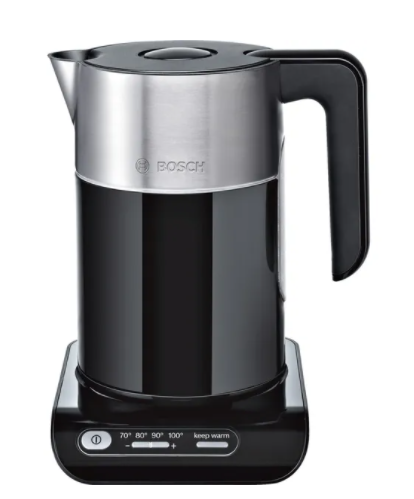
\includegraphics[height=4cm]{WK.png}
\column[t]{7cm}
$\SI{30}{\degreeCelsius}$ für eine Handwaschlauge, $\SI{40}{\degreeCelsius}$ für eine wohltuende Gesichtskompresse, $\SI{70}{\degreeCelsius}$ für einen aromatischen Grüntee, ... Oder sprudelnd kochend für einen schnellen Suppensnack. Jetzt erhitzen Sie Ihr Wasser immer exakt auf den Punkt. Und sparen Geld für unnötiges Aufheizen. Und Zeit fürs Abkühlen. \textbf{Sensor-Technik hält das Wasser auf Temperatur.}\\
\end{columns}
}
\frame
{
\frametitle{Beschreibung}
Per Knopfdruck aktivieren Sie die Sensor gesteuerte Warmhaltefunktion. Die automatische Endabschaltung verhindert eine Überhitzung des Kochers (sollte das Wasser einmal ganz verdunstet sein).\\
\textbf{Fast ca. $\SI{0.5}{\liter}$ mehr als die meisten anderen Kocher. }\\
$\SI{2300}{\watt}$ bringen in weniger als 6 Minuten $\SI{2}{\liter} $ zum Kochen. Aus mattiertem, rostfreiem Edelstahl. Hitze isolierender Griff. Sicherheitsdeckel mit Kalkfilter. Übersitzungsschutz. 360°-Sockel mit Kabelaufwicklung. 75cm-Anschlusskabel für $\SI{230}{\volt}$ / $\SI{2300}{\watt}$. GS-geprüfte Sicherheit. Misst 27 x 21 cm (H x \o). Wiegt ca. $\SI{1.7}{\kilogram}$. Herstellergarantie 2 Jahre.
}

\frame
{
\frametitle{Fragestellungen}
Können, wie in der Werbeanzeige behauptet, 2 Liter Wasser in weniger als 6 Minuten
zum Sieden gebracht werden?
\begin{enumerate}
\item Berechne erst die zum Erhitzen des Wassers von $\SI{30}{\celsius}$ auf $\SI{100}{\celsius}$ notwendige Energie!
\item Bestimme nun die zum Erhitzen erforderliche Zeit! Benutze hierzu die aus der Mechanik oder auch aus der Elektrizitätslehre bekannte Gleichung:\\


	\begin{exampleblock}{}
		{$ Leistung = \dfrac{Energie}{Zeit}$}
	\end{exampleblock}

\item Was kostet das Erhitzen des Wassers bei einem Kilowattstunden-preis von 28 Cent?
\end{enumerate}
}

\frame
{
  \frametitle{Wie viel Energie benötigt man, um eine Wassermenge um eine bestimmte Temperatur zu erhitzen?}
  
  \begin{alertblock}{Um 1 l Wasser um 1 K zu erhitzen, benötigt man eine Energie von 4,19 kJ.}
	  Es gilt:
  		\begin{equation}
  			c=\SI{4.19}{\dfrac{\kilo\joule}{\kilogram\cdot\kelvin}}
  		\end{equation}
  \end{alertblock}
  Um $\SI{2}{\liter}$ Wasser um $\SI{1}{\kelvin}$ zu erhitzen, benötigt man eine Energie von $2\cdot\SI{4.19}{\kilo\joule}\approx\SI{8.38}{\kilo\joule}$.\\
  Um $\SI{2}{\liter}$ Wasser um $\SI{70}{\kelvin}$ zu erhitzen, benötigt man eine Energie von $70\cdot\SI{8.38}{\kilo\joule}\approx\SI{587}{\kilo\joule}$.
}

\frame
{
  \frametitle{Lösung b)}
	\begin{exampleblock}{}
		\begin{equation}
			Leistung = \dfrac{Energie}{Zeit}\Rightarrow P=\dfrac{Q}{t}
		\end{equation}
	\end{exampleblock}
  \begin{align*}           
               \uncover<1->{&\Rightarrow t=\dfrac{Q}{P}}\\
               \uncover<2->{&\approx \dfrac{\SI{587}{\kilo\joule}}{\SI{2.3}{\kilo\watt}}=\dfrac{\SI{587}{\kilo\watt\second}}{\SI{2.3}{\kilo\watt}}}\\
               \uncover<3->{&\approx \SI{255}{\second}\approx \SI{4,25}{\minute}}\\
  \end{align*}
}

\frame
{
  \frametitle{Lösung c)}
  \begin{equation*}
  \SI{587}{\kilo\joule}=\SI{587}{\kilo\watt\second}=\dfrac{587}{3600} \si{\kilo\watt\hour}\approx\SI{0.16}{\kilo\watt\hour}
  \end{equation*}
  \setstretch{1.5}
	$\SI{1}{\kilo\watt\hour}$ kostet $0.28$ \euro \\
	$\SI{0.16}{\kilo\watt\hour}$ kosten ca. 4,6 Cent \\
  	Das Erwärmen des Wassers kostet ca. 4,6 Cent.
}

\end{document}